\chapter*{Практика 1. Знаковое кодирование}
\addcontentsline{toc}{chapter}{Практика 1. Знаковое кодирование}
\label{ch:1_practice}

\textit{\textbf{Задание:}} Реализовать знаковое кодирование и декодирование текстового сообщения.

\begin{itemize}
    \item Разработан кодер для преобразования текстового сообщения в битовую последовательность
    \item Каждый символ преобразуется в 8-битную последовательность
    \item Реализован декодер для обратного преобразования битов в текст
    \item Проведено тестирование корректности кодирования/декодирования
\end{itemize}

\begin{figure}[ht]
    \centering
    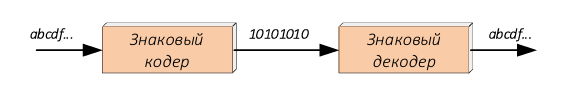
\includegraphics[width=0.8\textwidth]{symbolic_encoder_decoder.png}
    \caption{Блоксхема работы знакового кодера и декодера}
    \label{fig:symbolic_encoder_decoder}
\end{figure}

\begin{figure}[ht]
    \centering
    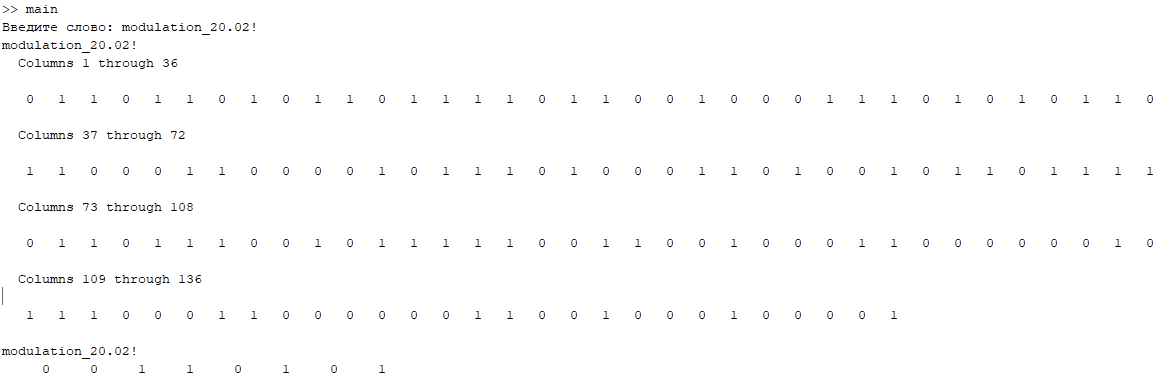
\includegraphics[width=0.8\textwidth]{1practice_result.png}
    \caption{Результат первой практики}
    \label{fig:1practice_result}
\end{figure}